\chapter{Specification}
\label{ch:spec}

This chapter defines what the system must do. It was written first as the requirement analysis of the first
milestone and extended as the project grew; the requirements below are the ones the final program implements.
Chapter~\ref{ch:test} shows, for each of them, the automated test that demonstrates it.

\section{Software perspective}

AK\&VEN is a new, self-contained web system: one server application with its database, and one web application that
runs in the browser and can be installed on a phone or a computer. It does not replace the stall; it extends it. The
stall remains the place where orders are collected and where the stock is kept, and the shop's data (the address of
the stall, the opening hours, the contacts, the prices and the size chart) is entered by the owners in the
administration rather than written into the code.

\section{User classes and characteristics}

\begin{table}[H]
	\centering
	\begin{tabularx}{\textwidth}{l X}
		\toprule
		\textbf{User} & \textbf{Description} \\
		\midrule
		Visitor & Anyone who opens the shop. Browses the catalogue, uses the size guide, the fitting room and the family
		planner, fills the bag, and sends a wholesale request, all without an account. \\
		Customer & A visitor with an account. Can also check out, ask the assistant for a better price, keep a family
		profile, saved socks and contact details, follow orders, write reviews and wait for sold-out options. \\
		Staff & An employee of the stall. Manages products, stock and orders, hands orders over at the stall, moderates
		reviews and answers wholesale requests; cannot change prices or the owners' limits. \\
		Owner (admin) & Akylbek and Venera. Everything staff can do, plus the limits per product, the price ladder, the
		exchange rates, delivery areas, contacts, opening hours, the size chart and customer accounts. \\
		Super admin & The person who runs the installation. Everything an owner can do, plus the team's accounts, the
		choice of assistant and the audit log. \\
		Assistant & Not a person: the negotiator called by the chat, either rule-based or a language model. Its
		behaviour and limits are part of the specification, not only of the implementation. \\
		Payment provider & The wallet (Apple Pay or Google Pay) that turns a card into a one-time token. Simulated in this
		thesis. \\
		\bottomrule
	\end{tabularx}
	\caption{Users of the system}
	\label{tab:users}
\end{table}

The customers are families and traders from Kyrgyzstan and the neighbouring countries. Many of them shop on a phone,
often with a weak connection, and read Russian or Kyrgyz more comfortably than English. The owners are not technical
users: the administration must use plain words, their language and few steps.

\section{Use cases}

Figures~\ref{fig:uc-customer} and~\ref{fig:uc-staff} show the use cases of the customer and of the shop team. The most
important one, \emph{Negotiate price}, involves the assistant as a secondary actor: the customer talks, the assistant
proposes, and the system decides.

\begin{figure}[H]
	\centering
	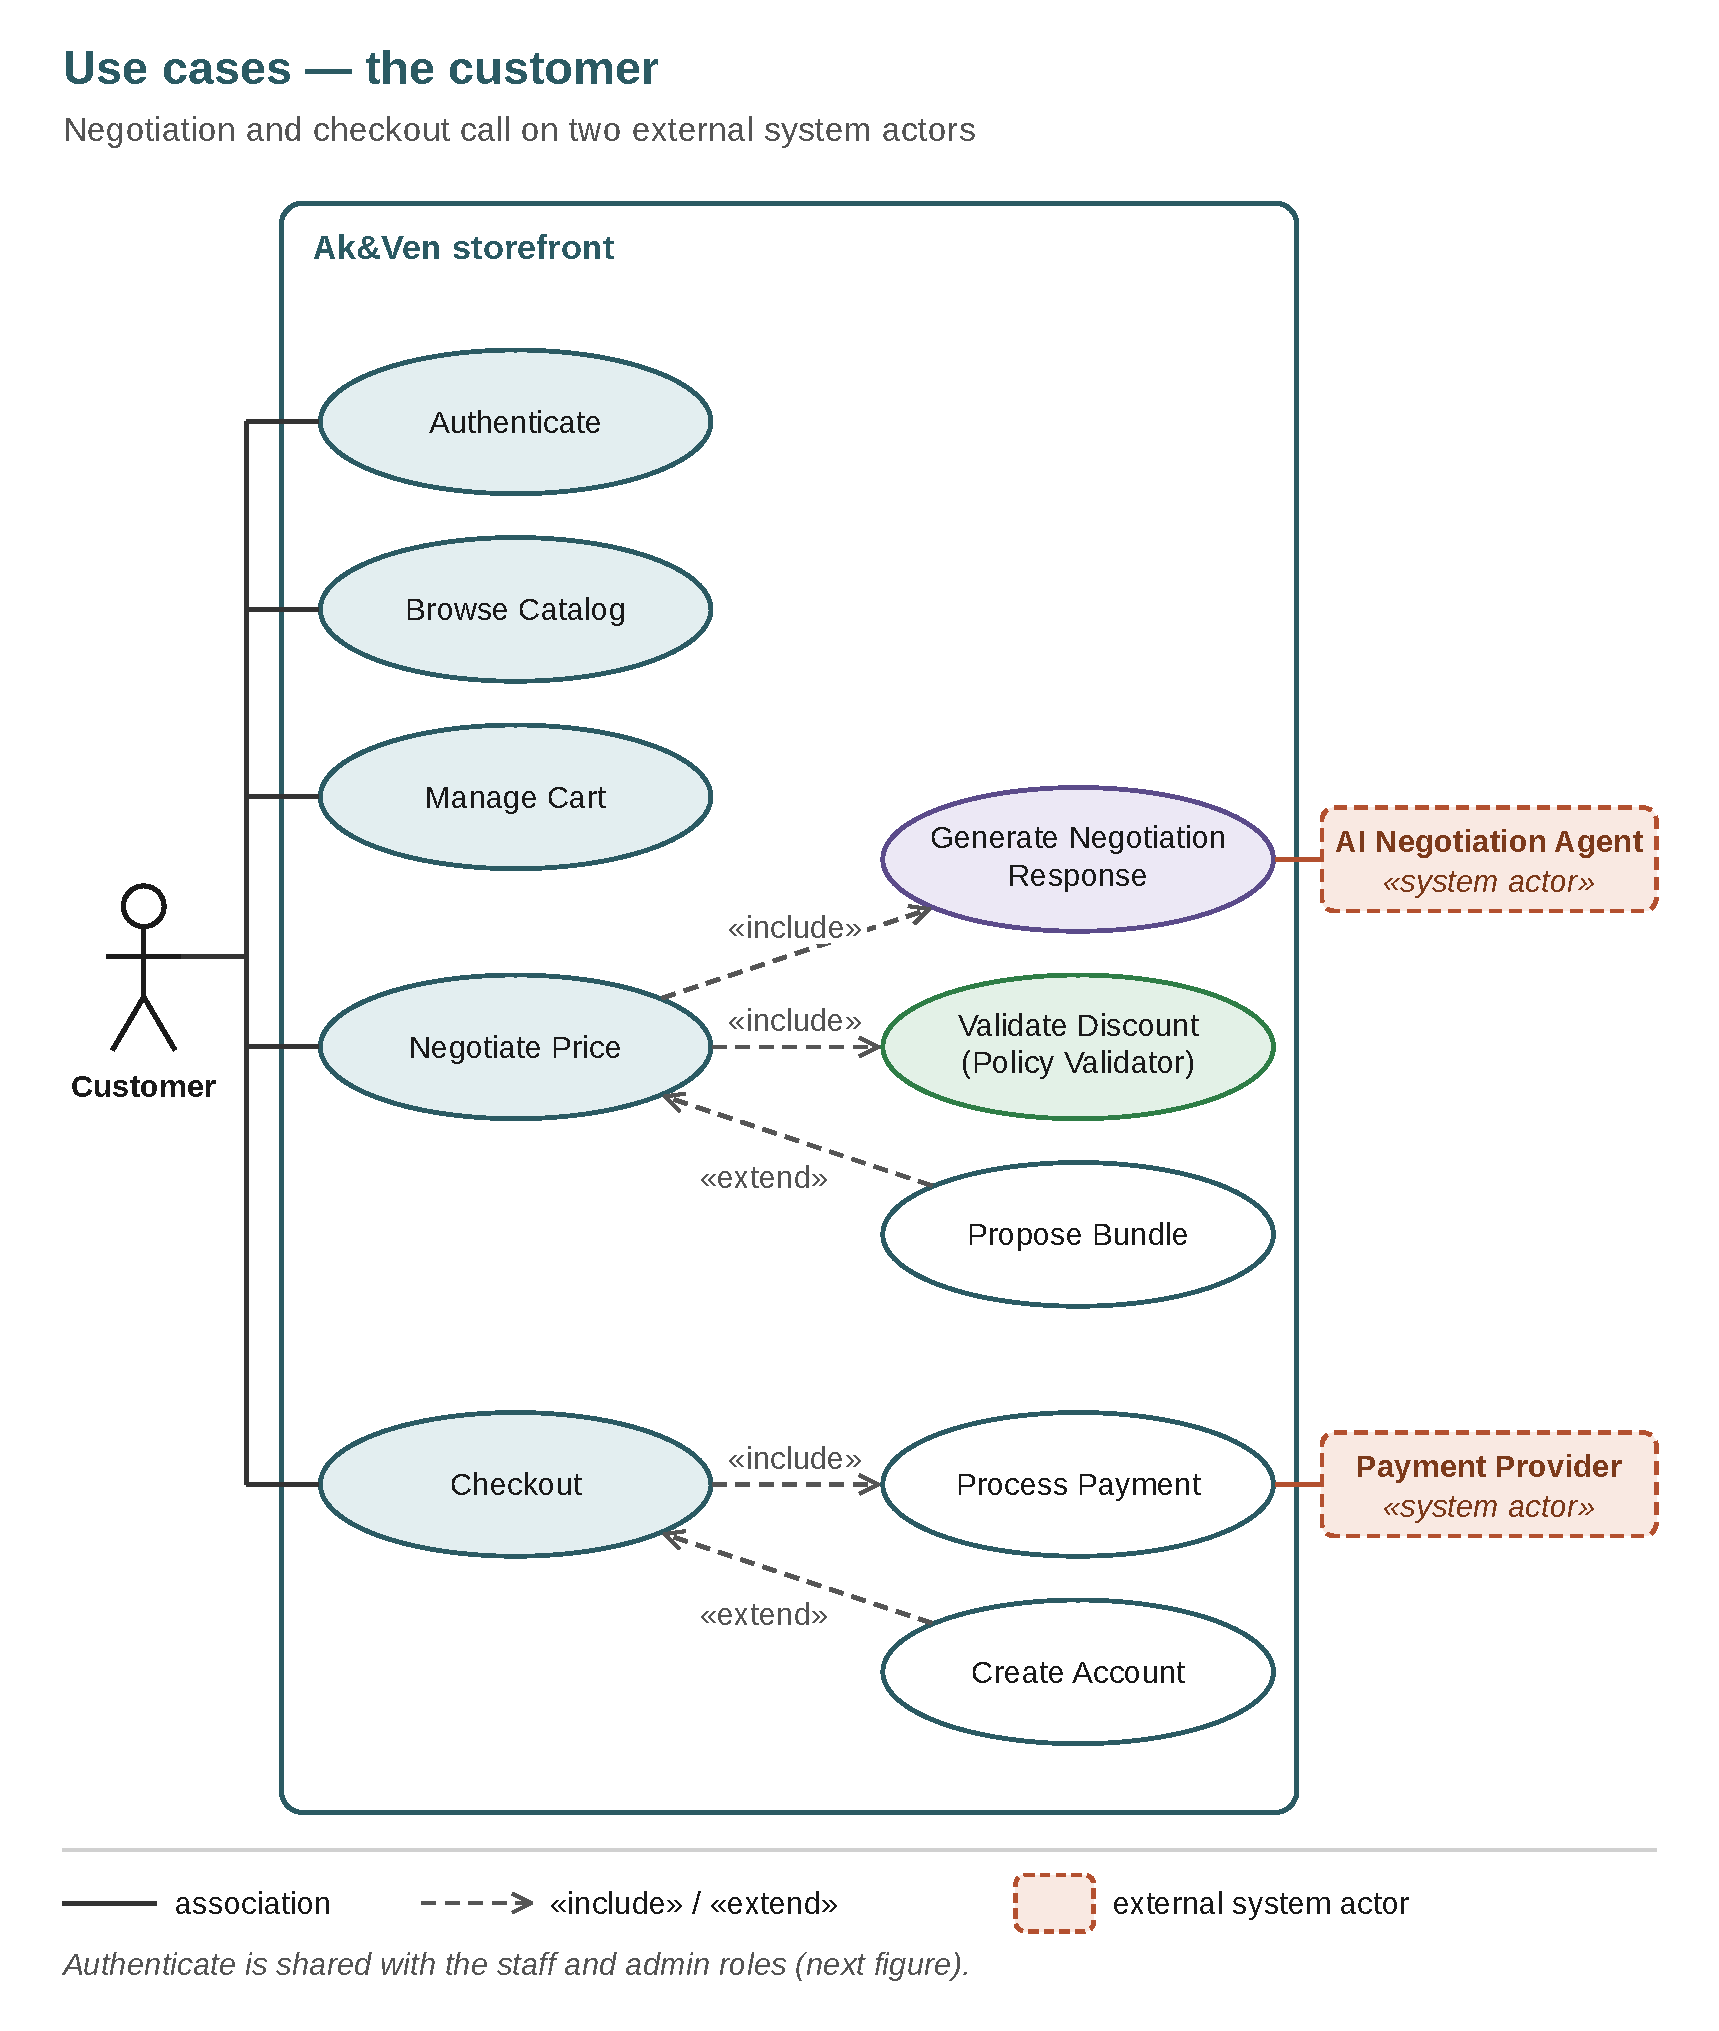
\includegraphics[width=0.92\textwidth]{05a-use-cases-customer.pdf}
	\caption{Use cases of visitors and customers}
	\label{fig:uc-customer}
\end{figure}

\begin{figure}[H]
	\centering
	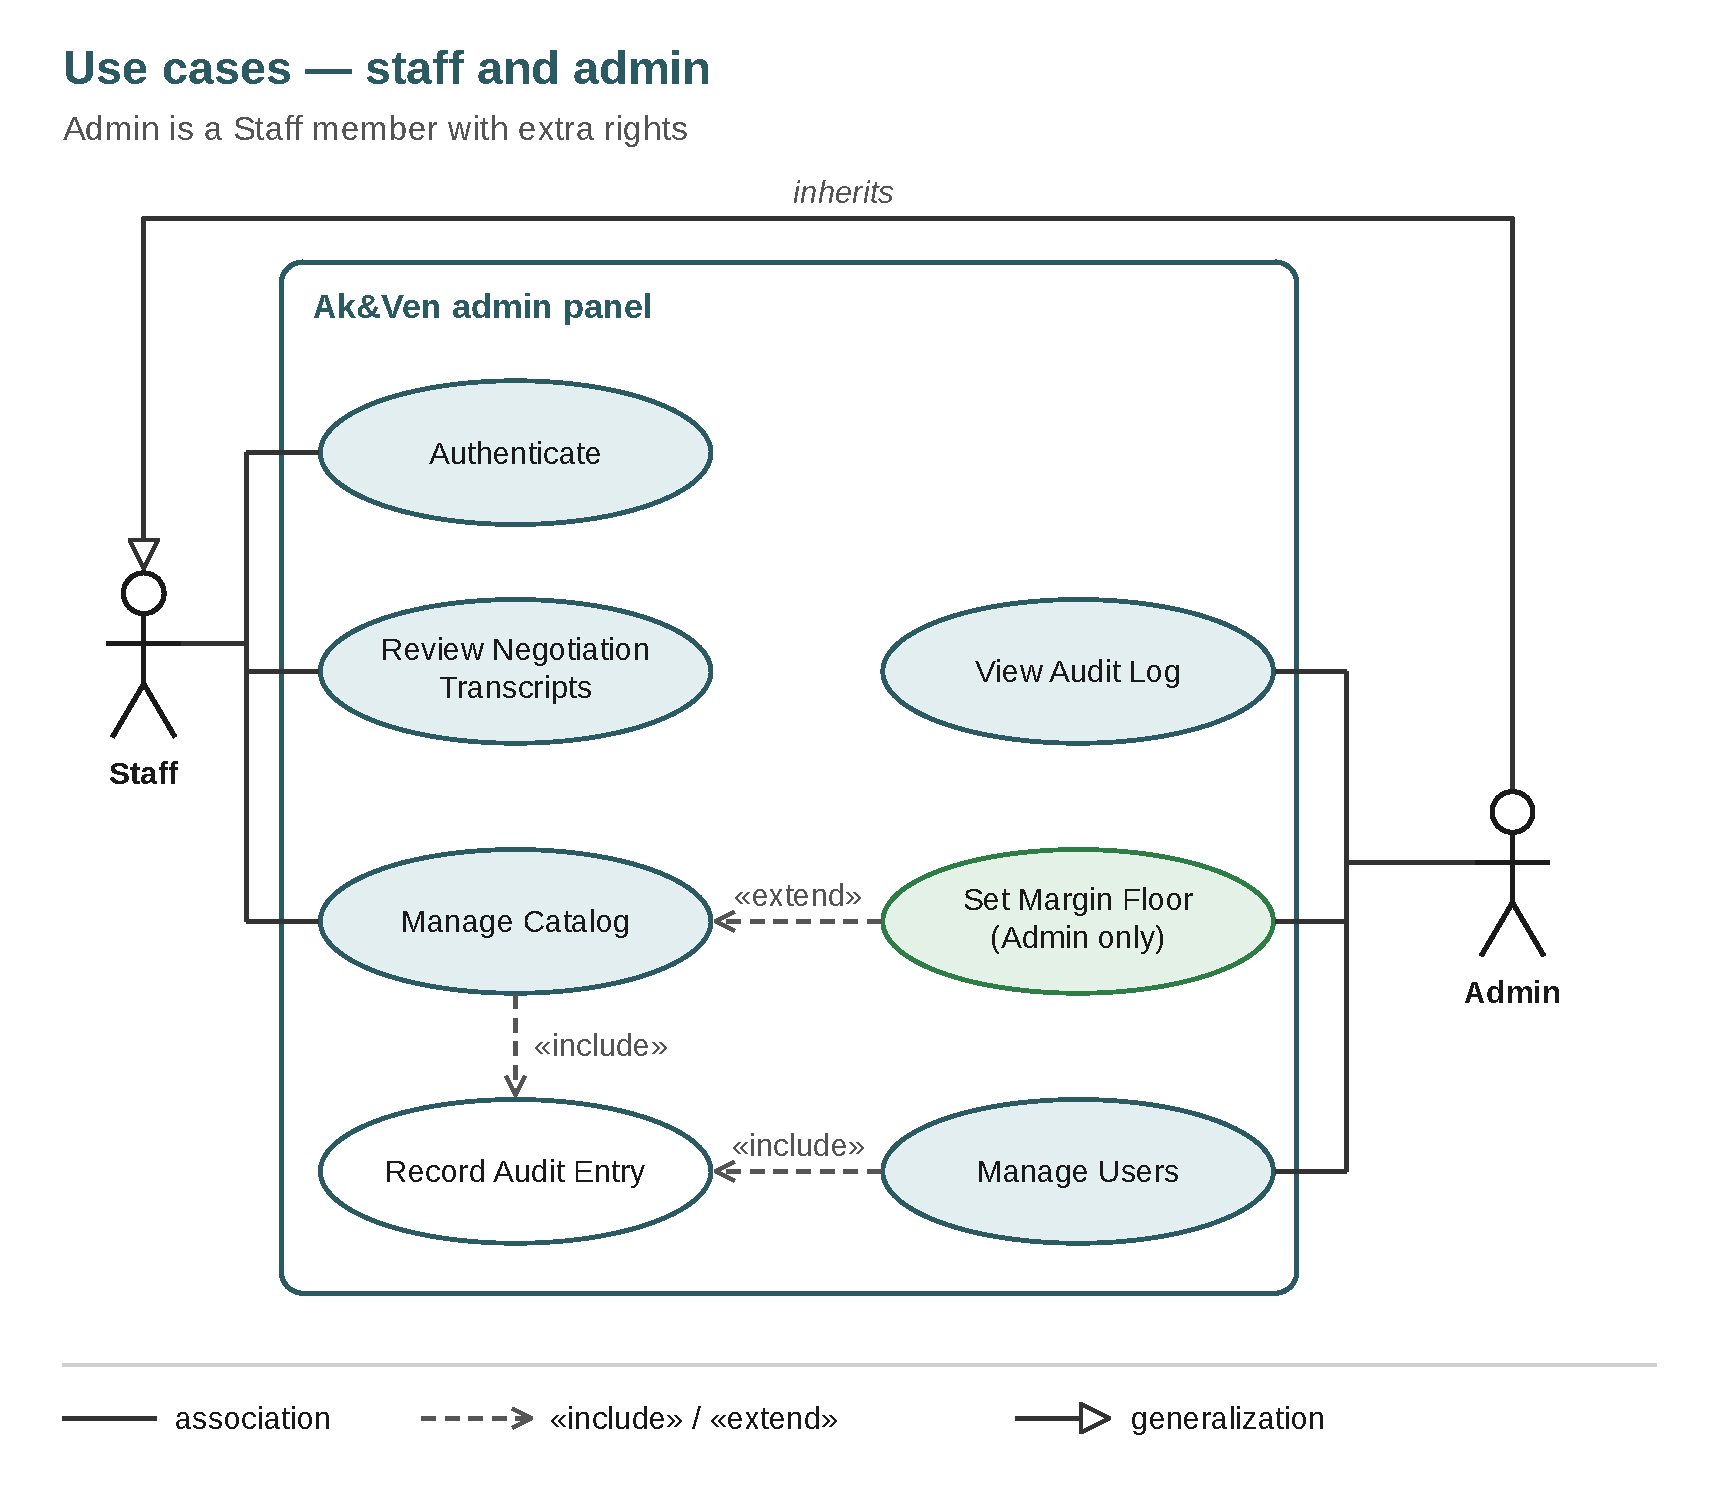
\includegraphics[width=0.92\textwidth]{05b-use-cases-staff-admin.pdf}
	\caption{Use cases of the staff, the owners and the super admin}
	\label{fig:uc-staff}
\end{figure}

\subsection{Representative scenarios}

\paragraph{A family set.} Aida needs socks for her husband (shoe size 43), herself (38) and her son (32). In the family
planner she adds the three of them; the shop works out the sock size of each from its own size chart and shows the
price step reached by the 15 pairs. She opens the shop with these sizes, fills the bag, pays with her phone's wallet and
receives a six-digit pickup code. At the stall she says the code and the last four digits of her phone number, and
Venera hands the bag over.

\paragraph{Bargaining.} A customer opens a sock and writes ``Can you do 50\% off for 10 pairs?''. The assistant answers
in the customer's language with an offer. Whatever it proposes, the offer shown is at most the limit the owners set
for that sock; it is kept for 24 hours, applies only to at least the negotiated number of pairs, and can be used once.

\paragraph{A shop from Osh.} A shop owner builds a case of 240 pairs from the shelves of men's, women's and children's
socks, writes the shop's name and a WhatsApp number, and sends the request. The shop answers with a reference number;
the request appears in the family's inbox, where they reply with one tap in the customer's own messenger.

\section{Functional requirements}

Table~\ref{tab:fr} lists the functional requirements. FR-1 to FR-14 come from the first milestone; FR-15 to FR-26
were added as the shop grew.

\begin{longtable}{p{1.4cm} p{12.6cm}}
	\toprule
	\textbf{ID} & \textbf{Requirement} \\
	\midrule
	\endhead
	FR-1 & List the products with their variants (size, colour, pack), price and stock, filterable by audience,
	section, cut, size, colour and stock. \\
	FR-2 & Let a visitor fill a bag without an account; the bag survives a reload and works offline. \\
	FR-3 & Accept a negotiation message about a product from a signed-in customer and return the assistant's answer,
	in the customer's language, as part of a conversation. \\
	FR-4 & Ground the assistant's answer in the product's real data (fabric, care, origin, pack, stock, price ladder),
	not in the model's general knowledge. \\
	FR-5 & Check every proposed discount with a deterministic validator against the product's limit before it can be
	shown, stored or charged; check it again at checkout. \\
	FR-6 & Record the proposed and the allowed discount of every negotiation. \\
	FR-7 & Take payment only through the wallet interface; never receive or store card numbers. \\
	FR-8 & Create a paid order only with a confirmed payment reference. \\
	FR-9 & Require authentication for staff and owner actions; staff cannot change prices or limits. \\
	FR-10 & Let the team create, edit, remove and restore products, variants, pictures and stock. \\
	FR-11 & Restrict cost price and limit changes to owners. \\
	FR-12 & Show the negotiations with both numbers, and a dashboard of offers, limits applied and sales. \\
	FR-13 & Record an audit entry (who, what, before, after) for every change to the catalogue, prices, orders,
	accounts and settings. \\
	FR-14 & Let the super admin manage the team's accounts and read the audit log. \\
	FR-15 & Price a bag as one collection: a minimum order and a ladder of discounts by the number of pairs in the whole
	bag, set by the owners. \\
	FR-16 & Offer pickup at the stall with a one-time code, and delivery to KG, KZ, UZ and RU by delivery areas with a
	fee, a free-from amount and a time, set by the owners. \\
	FR-17 & Let customers keep a family profile (names, roles, shoe sizes, birthdays) and derive the sock size from the
	shop's size chart. \\
	FR-18 & Let customers build a gift box (box, ribbon, card) that is packed at the stall. \\
	FR-19 & Accept reviews only from customers who received the product, and publish them after approval. \\
	FR-20 & Let customers wait for a sold-out option and show the owners who is waiting. \\
	FR-21 & Accept wholesale and company requests without an account, give a reference, and show them to the team in an
	inbox with statuses. \\
	FR-22 & Remember a customer's contact and delivery details on request, fill them in at checkout, and forget them on
	request. \\
	FR-23 & Show the shop, the administration and all messages in English, Russian and Kyrgyz, with prices in US
	dollars, Kyrgyz som or Russian roubles at rates the owners set. \\
	FR-24 & Show whether the stall is open now in Bishkek time, its hours and how to find it. \\
	FR-25 & Let the super admin switch the assistant between the rules and the language model at run time, try it, and
	repeat the evaluation. \\
	FR-26 & Export the orders of a period as a spreadsheet file for the owners. \\
	\bottomrule
	\caption{Functional requirements}
	\label{tab:fr}
\end{longtable}

\section{Non-functional requirements}

\begin{longtable}{p{1.4cm} p{2.9cm} p{9.2cm}}
	\toprule
	\textbf{ID} & \textbf{Category} & \textbf{Requirement} \\
	\midrule
	\endhead
	NFR-1 & Security & Passwords are stored only as BCrypt hashes. \\
	NFR-2 & Security & Every endpoint enforces the roles; there is one API, not a separate administration backend. \\
	NFR-3 & Security & Customer text sent to the assistant is untrusted; no discount reaches an order without the
	validator. \\
	NFR-4 & Security & No card data is received, stored or logged. \\
	NFR-5 & Reliability & The bag works offline; prices are always recomputed by the server. \\
	NFR-6 & Performance & An assistant answer arrives within a conversational time (target: under about 5 seconds). \\
	NFR-7 & Maintainability & Every change by the team can be reconstructed from the audit log alone. \\
	NFR-8 & Testability & The validator and the pricing are testable without the language model; the build fails
	under 80\% line coverage. \\
	NFR-9 & Portability & One installable PWA serves customers and the team through role-gated routes. \\
	NFR-10 & Operability & Build and tests run automatically in CI on every push. \\
	NFR-11 & Usability & The shop works on phones, tablets and laptops; text meets WCAG 2.2 AA contrast; pages pass
	automated accessibility rules. \\
	NFR-12 & Integrity & The most important rules (stock never below zero, an allowed discount never above its proposal,
	a paid order has a payment reference) are also enforced by database constraints. \\
	\bottomrule
	\caption{Non-functional requirements}
	\label{tab:nfr}
\end{longtable}

\section{Constraints}

\begin{itemize}
	\item \textbf{Technology:} Java 17 and Spring Boot 3.3 for the server, PostgreSQL 16 with pgvector for the data,
	React 18 with TypeScript for the client, Docker Compose for running the whole system.
	\item \textbf{Time:} the ELTE milestones (requirements on 25 September, prototype on 20 October, final program on
	10 November, draft on 22 November, submission on 1 December 2026).
	\item \textbf{Business:} there is no agreement with a Kyrgyz payment provider, so payment goes through a wallet
	interface with a simulated implementation; no real money moves.
	\item \textbf{Privacy:} real phone numbers, passwords and API keys are never written into the repository; they come
	from the environment of each installation.
\end{itemize}

\section{Assumptions and dependencies}

\begin{itemize}
	\item A language model with an OpenAI-compatible chat API is available (Gemini by default~\cite{gemini}). Without a
	key, the rule-based assistant answers, so the shop never depends on the model.
	\item The demo catalogue (about 220 products with over 1,200 options) is drawn by the project itself until the family
	photographs the real products; the drawings use the same sock shapes and colours as the brand.
	\item Prices, limits, delivery fees and times in the demo are examples; the owners enter the real ones.
\end{itemize}

\section{User interface plan}

The interface was planned as wireframes for the five key screens (catalogue, product with the bag, checkout, the
negotiation chat and the administration dashboard) on a phone, a tablet and a laptop before it was built; the final
design keeps that structure. Its visual language comes from the stall itself (Section~\ref{sec:design}): kraft price
tags, the family's handwriting, socks hanging on a washing line, and container 70-E.
